%!TEX root = ../root.tex

Let us recap briefly what is the general setting:
in deep learning, we deal with \emph{highly parametrized} models, usually in the order of millions or even hundreds of millions of parameters, and these models are called \emph{deep neural networks}. A deep neural network models some function $f$, possibly nonlinear, parametrized by parameters $\Theta$. In general, given a data point $x$ in input to the neural network, this returns an output $y$:

\begin{equation}
	f_{\Vector{\Theta}}(\vec{x}) = \vec{y}
\end{equation}

A neural network takes the form of a composition of multiple simpler blocks each of which has a predefined structure (\textit{e.g.} one block might be modelling a linear map). The structure is chosen by who designs the neural network, so this is not something that we solve for, but is fixed during the design of the neural network.

Each block is defined in terms of unknown parameters $\Theta$ and the collection of the parameters of all the blocks are the parameters of the entire network.

\begin{figure}[H]
	\centering
	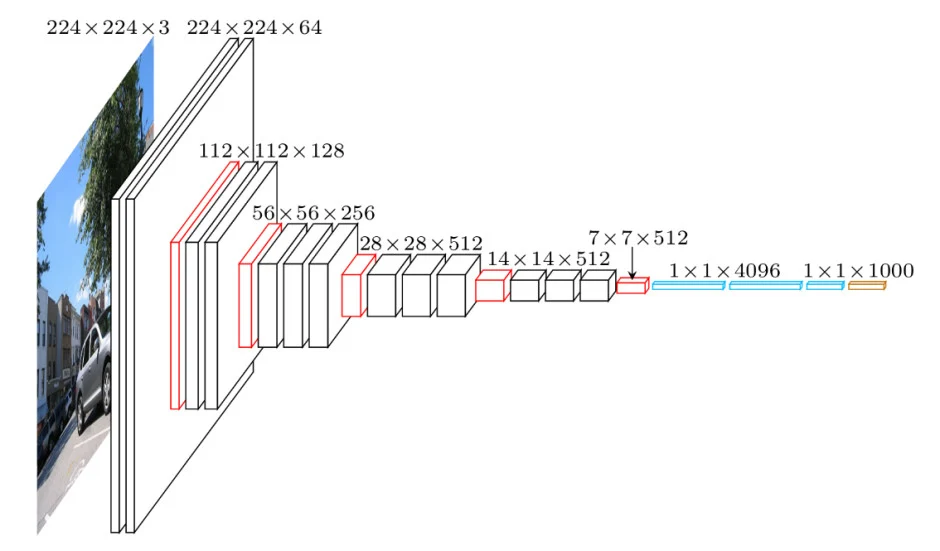
\includegraphics[width=.5\textwidth]{04/nn1}
	\caption{Example of a neural network structure}\label{fig:nn-structure}	
\end{figure}

We usually have access to few data points $X$ and a few data points $Y$, \textit{i.e.} our training pairs of examples, and our task is to solve for the parameters $\Theta$ of the function $f_{\vb*{\Theta}}$ that \emph{is most likely} to have produced $Y$ from $X$, i.e. we have to \emph{infer} the function $f$ from $\{X, Y\}$. Finding the values of the function parameters $\vb*{\Theta}$ is called \emph{training}. 

In order to do this, we need to define some criterion with which we can say that the \emph{learned function} $f_{\vb*{\Theta}}$ is more or less likely to represent \emph{true function} $f$. This is usually done by defining some energy function that depends on the produced output $\hat{Y} = f_{\vb*{\Theta}}(X)$, and so indirectly on the parameters $\vb*{\Theta}$ (since these influence the learned function $f_{\vb*{\Theta}}$), that we usually call \emph{loss function}, which we want to minimize. 
Finding the parameters that minimize the loss function will be done using an optimization procedure that requires computing gradients, so it involves what we call \emph{backpropagation}, \textit{i.e.} the process of computing derivatives of all the functions involved in the network.

\section{Linear Regression} 
%!TEX root=../../../root.tex

Consider a linear map $T:V \to W$, a basis $v_1,\dots,v_n \in V$ and a basis $w_1,\dots,w_m\in W$.
{
The \emph{matrix} of $T$ in these bases is the $m\times n$ array of values in $\mathbb{R}$
%
\[
\mathbf{T} = \begin{pmatrix}
    T_{1,1} & \cdots & T_{1,n} \\
    \vdots & & \vdots\\
    T_{m,1} & \cdots & T_{m,n}
  \end{pmatrix}
\]
%
whose entries $T_{i,j}$ are defined by
%
\[
{\color{darkgreen}Tv_j} = {\color{red}T_{1,j}} w_1 + \cdots + {\color{red}T_{m,j}} w_m
\]
}%

{
Hence each column of $\mathbf{T}$ contains the {\color{red}linear combination coefficients} for the {\color{darkgreen}image via $T$ of a basis vector from $V$}
}

{
In other words, the matrix encodes {\color{darkgreen}how basis vectors are mapped}, and this is enough to map all other vectors in their span, since:
\[ Tv = T ( \sum_j \alpha_j v_j ) = \sum_j T(\alpha_j v_j) = \sum_j \alpha_j {\color{darkgreen}Tv_j} \]
}

The matrix is a \emph{representation} for a linear map, and it \emph{depends on the choice of bases}.
Suppose $v \in V$ is an arbitrary vector, while $v_1,\dots,v_n$ is a basis of $V$. The matrix of $v$ wrt this basis is the $n\times 1$ matrix:
%
\[
\mathbf{v} = \begin{pmatrix}
    c_1 \\
    \vdots\\
    c_n
  \end{pmatrix}
\]
%
so that
%
\[
v = c_1 v_1 + \cdots c_n v_n
\]

Once again, we see that the matrix \emph{depends on the choice of basis} for $V$


\begin{itemize}
\item \textbf{addition}:  the matrix of $S+T$ can be obtained by summing the matrices of $S$ and $T${; this only makes sense if the \emph{same bases} are used for $S$, $T$, and $S+T$}
\item \textbf{scalar multiplication}: given $\lambda\in\mathbb{R}$, the matrix for $\lambda T$ is given by $\lambda$ times the matrix of $T$
\end{itemize}

{
In fact, we have just shown that \emph{matrices form a vector space} (Q1: what is the additive identity?) {(Q2: what is the vector space dimension?)}
}

{
We call $\mathbb{R}^{m\times n}$ the vector space of all $m\times n$ matrices with values in $\mathbb{R}$
}

{
\begin{itemize}
\item \textbf{product}: the matrix for $ST$ can be computed by the \emph{matrix product} between $\mathbf{S}$ and $\mathbf{T}$; in fact, the matrix product is defined precisely to make this work

{
Q3: is matrix product commutative?
}

{
Q4: do we need the same bases for $S:U\to V$ and $T:V \to W$?
}

\end{itemize}
}



Consider a linear map $T:V \to W$, a basis $v_1,\dots,v_n \in V$ and a basis $w_1,\dots,w_m\in W$.

%\medskip
%The $k$-th column of $\mathbf{T}$ equals the matrix vector $\mathbf{v}_k$:

%figure

From the definition of matrix product, one can show that it operates on a vector matrix as expected:
\[
\mathbf{Tv} =\mathbf{w} \quad \Leftrightarrow \quad Tv=w
\]
where $\mathbf{Tv}$ is the matrix product of $\mathbf{T}$ and $\mathbf{v}$, while $Tv$ simply denotes the function evaluation $T(v)$


{
\textbf{Remember:} $\mathbf{T}, \mathbf{v}, \mathbf{w}$ must follow a coherent choice of bases in order for the above to make sense. $\mathbf{v}$ can not be expressed in basis $\color{red}(\tilde{v}_1,\dots,\tilde{v}_n)$ if $\mathbf{T}$ only knows how to map basis vectors $\color{blue}({v}_1,\dots,{v}_n)$.
%
\[
T{\color{blue}v_j} = {\color{blue}T_{1,j}} w_1 + \cdots + {\color{blue}T_{m,j}} w_m
\]
%
%\[ Tv =  \sum_j \alpha_j T{\color{red}\tilde{v}_j} \]
}


\[
\underbrace{
\begin{pmatrix}
    T_{1,1} & \cdots & T_{1,n} \\
    \vdots & & \vdots\\
    T_{m,1} & \cdots & T_{m,n}
  \end{pmatrix}}_{\mathbf{T}}
  %
  \underbrace{
  \begin{pmatrix}
    c_1 \\
    \vdots \\
    c_n
  \end{pmatrix}}_{\mathbf{c}} =
  %
   \sum_{j=1}^n c_j \hspace{-0.6cm}
   \underbrace{\begin{pmatrix}
    {\color{red}T_{1,j}}  \\
    \vdots \\
    {\color{red}T_{m,j}}
  \end{pmatrix}}_{\mathrm{Tv_j~wrt~(w_1,\dots,w_m)}}
\]
%
\smallskip

Because recall that, for bases $v_1,\dots,v_n \in V$ and $w_1,\dots,w_m\in W$:
%
\[
Tv_j = {\color{red}T_{1,j}} w_1 + \cdots + {\color{red}T_{m,j}} w_m
\]

{
We see then that vector $c=\sum_j c_j v_j$ is mapped to $Tc = \sum_j c_j Tv_j$.

In other words, matrix product is behaving as expected.
}








\section{Convexity} 
%!TEX root=../../../root.tex

Consider a linear map $T:V \to W$, a basis $v_1,\dots,v_n \in V$ and a basis $w_1,\dots,w_m\in W$.
{
The \emph{matrix} of $T$ in these bases is the $m\times n$ array of values in $\mathbb{R}$
%
\[
\mathbf{T} = \begin{pmatrix}
    T_{1,1} & \cdots & T_{1,n} \\
    \vdots & & \vdots\\
    T_{m,1} & \cdots & T_{m,n}
  \end{pmatrix}
\]
%
whose entries $T_{i,j}$ are defined by
%
\[
{\color{darkgreen}Tv_j} = {\color{red}T_{1,j}} w_1 + \cdots + {\color{red}T_{m,j}} w_m
\]
}%

{
Hence each column of $\mathbf{T}$ contains the {\color{red}linear combination coefficients} for the {\color{darkgreen}image via $T$ of a basis vector from $V$}
}

{
In other words, the matrix encodes {\color{darkgreen}how basis vectors are mapped}, and this is enough to map all other vectors in their span, since:
\[ Tv = T ( \sum_j \alpha_j v_j ) = \sum_j T(\alpha_j v_j) = \sum_j \alpha_j {\color{darkgreen}Tv_j} \]
}

The matrix is a \emph{representation} for a linear map, and it \emph{depends on the choice of bases}.
Suppose $v \in V$ is an arbitrary vector, while $v_1,\dots,v_n$ is a basis of $V$. The matrix of $v$ wrt this basis is the $n\times 1$ matrix:
%
\[
\mathbf{v} = \begin{pmatrix}
    c_1 \\
    \vdots\\
    c_n
  \end{pmatrix}
\]
%
so that
%
\[
v = c_1 v_1 + \cdots c_n v_n
\]

Once again, we see that the matrix \emph{depends on the choice of basis} for $V$


\begin{itemize}
\item \textbf{addition}:  the matrix of $S+T$ can be obtained by summing the matrices of $S$ and $T${; this only makes sense if the \emph{same bases} are used for $S$, $T$, and $S+T$}
\item \textbf{scalar multiplication}: given $\lambda\in\mathbb{R}$, the matrix for $\lambda T$ is given by $\lambda$ times the matrix of $T$
\end{itemize}

{
In fact, we have just shown that \emph{matrices form a vector space} (Q1: what is the additive identity?) {(Q2: what is the vector space dimension?)}
}

{
We call $\mathbb{R}^{m\times n}$ the vector space of all $m\times n$ matrices with values in $\mathbb{R}$
}

{
\begin{itemize}
\item \textbf{product}: the matrix for $ST$ can be computed by the \emph{matrix product} between $\mathbf{S}$ and $\mathbf{T}$; in fact, the matrix product is defined precisely to make this work

{
Q3: is matrix product commutative?
}

{
Q4: do we need the same bases for $S:U\to V$ and $T:V \to W$?
}

\end{itemize}
}



Consider a linear map $T:V \to W$, a basis $v_1,\dots,v_n \in V$ and a basis $w_1,\dots,w_m\in W$.

%\medskip
%The $k$-th column of $\mathbf{T}$ equals the matrix vector $\mathbf{v}_k$:

%figure

From the definition of matrix product, one can show that it operates on a vector matrix as expected:
\[
\mathbf{Tv} =\mathbf{w} \quad \Leftrightarrow \quad Tv=w
\]
where $\mathbf{Tv}$ is the matrix product of $\mathbf{T}$ and $\mathbf{v}$, while $Tv$ simply denotes the function evaluation $T(v)$


{
\textbf{Remember:} $\mathbf{T}, \mathbf{v}, \mathbf{w}$ must follow a coherent choice of bases in order for the above to make sense. $\mathbf{v}$ can not be expressed in basis $\color{red}(\tilde{v}_1,\dots,\tilde{v}_n)$ if $\mathbf{T}$ only knows how to map basis vectors $\color{blue}({v}_1,\dots,{v}_n)$.
%
\[
T{\color{blue}v_j} = {\color{blue}T_{1,j}} w_1 + \cdots + {\color{blue}T_{m,j}} w_m
\]
%
%\[ Tv =  \sum_j \alpha_j T{\color{red}\tilde{v}_j} \]
}


\[
\underbrace{
\begin{pmatrix}
    T_{1,1} & \cdots & T_{1,n} \\
    \vdots & & \vdots\\
    T_{m,1} & \cdots & T_{m,n}
  \end{pmatrix}}_{\mathbf{T}}
  %
  \underbrace{
  \begin{pmatrix}
    c_1 \\
    \vdots \\
    c_n
  \end{pmatrix}}_{\mathbf{c}} =
  %
   \sum_{j=1}^n c_j \hspace{-0.6cm}
   \underbrace{\begin{pmatrix}
    {\color{red}T_{1,j}}  \\
    \vdots \\
    {\color{red}T_{m,j}}
  \end{pmatrix}}_{\mathrm{Tv_j~wrt~(w_1,\dots,w_m)}}
\]
%
\smallskip

Because recall that, for bases $v_1,\dots,v_n \in V$ and $w_1,\dots,w_m\in W$:
%
\[
Tv_j = {\color{red}T_{1,j}} w_1 + \cdots + {\color{red}T_{m,j}} w_m
\]

{
We see then that vector $c=\sum_j c_j v_j$ is mapped to $Tc = \sum_j c_j Tv_j$.

In other words, matrix product is behaving as expected.
}








\section{Gradients} 
%!TEX root=../../../root.tex

Consider a linear map $T:V \to W$, a basis $v_1,\dots,v_n \in V$ and a basis $w_1,\dots,w_m\in W$.
{
The \emph{matrix} of $T$ in these bases is the $m\times n$ array of values in $\mathbb{R}$
%
\[
\mathbf{T} = \begin{pmatrix}
    T_{1,1} & \cdots & T_{1,n} \\
    \vdots & & \vdots\\
    T_{m,1} & \cdots & T_{m,n}
  \end{pmatrix}
\]
%
whose entries $T_{i,j}$ are defined by
%
\[
{\color{darkgreen}Tv_j} = {\color{red}T_{1,j}} w_1 + \cdots + {\color{red}T_{m,j}} w_m
\]
}%

{
Hence each column of $\mathbf{T}$ contains the {\color{red}linear combination coefficients} for the {\color{darkgreen}image via $T$ of a basis vector from $V$}
}

{
In other words, the matrix encodes {\color{darkgreen}how basis vectors are mapped}, and this is enough to map all other vectors in their span, since:
\[ Tv = T ( \sum_j \alpha_j v_j ) = \sum_j T(\alpha_j v_j) = \sum_j \alpha_j {\color{darkgreen}Tv_j} \]
}

The matrix is a \emph{representation} for a linear map, and it \emph{depends on the choice of bases}.
Suppose $v \in V$ is an arbitrary vector, while $v_1,\dots,v_n$ is a basis of $V$. The matrix of $v$ wrt this basis is the $n\times 1$ matrix:
%
\[
\mathbf{v} = \begin{pmatrix}
    c_1 \\
    \vdots\\
    c_n
  \end{pmatrix}
\]
%
so that
%
\[
v = c_1 v_1 + \cdots c_n v_n
\]

Once again, we see that the matrix \emph{depends on the choice of basis} for $V$


\begin{itemize}
\item \textbf{addition}:  the matrix of $S+T$ can be obtained by summing the matrices of $S$ and $T${; this only makes sense if the \emph{same bases} are used for $S$, $T$, and $S+T$}
\item \textbf{scalar multiplication}: given $\lambda\in\mathbb{R}$, the matrix for $\lambda T$ is given by $\lambda$ times the matrix of $T$
\end{itemize}

{
In fact, we have just shown that \emph{matrices form a vector space} (Q1: what is the additive identity?) {(Q2: what is the vector space dimension?)}
}

{
We call $\mathbb{R}^{m\times n}$ the vector space of all $m\times n$ matrices with values in $\mathbb{R}$
}

{
\begin{itemize}
\item \textbf{product}: the matrix for $ST$ can be computed by the \emph{matrix product} between $\mathbf{S}$ and $\mathbf{T}$; in fact, the matrix product is defined precisely to make this work

{
Q3: is matrix product commutative?
}

{
Q4: do we need the same bases for $S:U\to V$ and $T:V \to W$?
}

\end{itemize}
}



Consider a linear map $T:V \to W$, a basis $v_1,\dots,v_n \in V$ and a basis $w_1,\dots,w_m\in W$.

%\medskip
%The $k$-th column of $\mathbf{T}$ equals the matrix vector $\mathbf{v}_k$:

%figure

From the definition of matrix product, one can show that it operates on a vector matrix as expected:
\[
\mathbf{Tv} =\mathbf{w} \quad \Leftrightarrow \quad Tv=w
\]
where $\mathbf{Tv}$ is the matrix product of $\mathbf{T}$ and $\mathbf{v}$, while $Tv$ simply denotes the function evaluation $T(v)$


{
\textbf{Remember:} $\mathbf{T}, \mathbf{v}, \mathbf{w}$ must follow a coherent choice of bases in order for the above to make sense. $\mathbf{v}$ can not be expressed in basis $\color{red}(\tilde{v}_1,\dots,\tilde{v}_n)$ if $\mathbf{T}$ only knows how to map basis vectors $\color{blue}({v}_1,\dots,{v}_n)$.
%
\[
T{\color{blue}v_j} = {\color{blue}T_{1,j}} w_1 + \cdots + {\color{blue}T_{m,j}} w_m
\]
%
%\[ Tv =  \sum_j \alpha_j T{\color{red}\tilde{v}_j} \]
}


\[
\underbrace{
\begin{pmatrix}
    T_{1,1} & \cdots & T_{1,n} \\
    \vdots & & \vdots\\
    T_{m,1} & \cdots & T_{m,n}
  \end{pmatrix}}_{\mathbf{T}}
  %
  \underbrace{
  \begin{pmatrix}
    c_1 \\
    \vdots \\
    c_n
  \end{pmatrix}}_{\mathbf{c}} =
  %
   \sum_{j=1}^n c_j \hspace{-0.6cm}
   \underbrace{\begin{pmatrix}
    {\color{red}T_{1,j}}  \\
    \vdots \\
    {\color{red}T_{m,j}}
  \end{pmatrix}}_{\mathrm{Tv_j~wrt~(w_1,\dots,w_m)}}
\]
%
\smallskip

Because recall that, for bases $v_1,\dots,v_n \in V$ and $w_1,\dots,w_m\in W$:
%
\[
Tv_j = {\color{red}T_{1,j}} w_1 + \cdots + {\color{red}T_{m,j}} w_m
\]

{
We see then that vector $c=\sum_j c_j v_j$ is mapped to $Tc = \sum_j c_j Tv_j$.

In other words, matrix product is behaving as expected.
}








